\documentclass[a4paper,12pt]{report}
\usepackage{graphicx}
\title{Tugas pemrograman Chapter 2}
\author{Nuha Hanifatul Khonsa'}
\date{24 oktober 2019}
\begin{document}


\maketitle


\section{Teori}
\subsection{Variable}
\usepackage{Variable adalah sebuah wadah yang memiliki nilai. Variable dapat dituliskan dengan sederhana seperti berikut: dimana nama variable = nilai. jika nama variable diisi npm maka nilai yang dimasukkan ialah 1184085.  Dalam variable exsplorer pada Python berisikan nama, type data serta value dari variable yang ada dalam syntax Python}

\subsection{Input dan Output}
\usepackage{Input dalam Python adalah sebuah masukan dari user kemudian diproses kepada program dan program memberikan output pada user. Input dan Output ialah hal paling penting dari sebuah program. 
inputan bisa dari value dari sebuah variable dan output adalah print atau hasil dari nilai sebuah variable. }

\susection{Operator Dasar Aritmatika}
\usepackage{Operator aritmatika adalah simbol aritmatika yang berlaku dalam Python, Sama halnya dengan operator aritmatika lain yang ada seprti jumlah, bagi, kurang, kali, dll,}
\begin{center}
        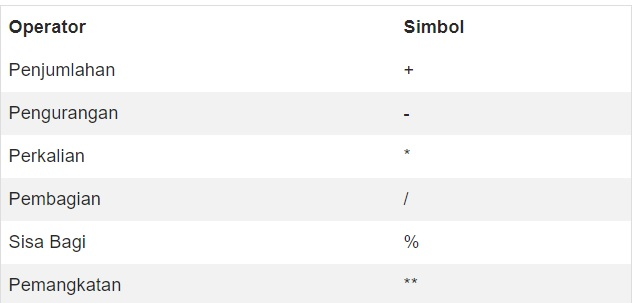
\includegraphics[width=8cm\textwidth]{aritmatika.jpg}
\end{center}

\textbf{Fungsi-fungsi untuk mengubah tipe data:}
\begin{enumerate}
    \item int() untuk mengubah menjadi integer;
    \item long() untuk mengubah menjadi integer panjang;
    \item float() untuk mengubah menjadi float;
    \item bool() untuk mengubah menjadi boolean;
    \item chr() untuk mengubah menjadi karakter;
    \item str() untuk mengubah menjadi string.
    \item bin() untuk mengubah menjadi bilangan Biner.
    \item hex() untuk mengubah menjadi bilangan Heksadesimal.
    \item oct() untuk mengubah menjadi bilangan okta.
\end{enumerate}

\subsection{Syntax Perulangan}
\begin{enumerate}
    \item For
    \begin{itemize}
        \item Perulangan menggunakan for dimana perulangan akan terus berulang sampai batas yang ditentukan.
    \end{itemize}
    \begin{verbatim}
        ulang = 87
        for i in range(ulang):
        print(" halo " +npm+ " apa kabar" )
    \end{verbatim}
    \item While
    \begin{itemize}
        \item Perulangan dengan t kondisi benar atau salah. 
    \end{itemize}
    \begin{verbatim}
        jawab = 'ya'
        hitung = 0

        while(True):
           hitung += 1
           jawab = raw_input("Ulang lagi tidak? ")
          if jawab == 'tidak':
            break

        print "Total perulagan: " + str(hitung)
    \end{verbatim}
    \item If
    \begin{itemize}
        \item Kondisi dimana terdapat 2 keaadaan dimana jika benar dengan aksi tertentu\\
        If(kondisi):\\
        Aksi\\
        \begin{verbatim}
        a=5
        if a > 3:
        print "angka lebih besar dari 3"
        \end{verbatim}
    \end{itemize}
    \item If Else
    \begin{itemize}
        \item Kondisi dimana if adalah keadaan dimana jika benar maka ada aksi dan jika salah maka aksi akan dilakukan pada else\\
            If(kondisi):\\
            Aksi1\\
            Else\\
            Aksi2\\
        \begin{verbatim}
            a=5
            if a > 3:
                print("angka lebih besar dari 3")
            else:
                print("angka kurang dari 3")
        \end{verbatim}
    \end{itemize}
\end{enumerate}


\subsection{Eror pada Python}
\subsection{Try Except}

\section{Keterampilan Pemrograman}
\begin{enumerate}
    \item Soal 1
    \begin{center}
    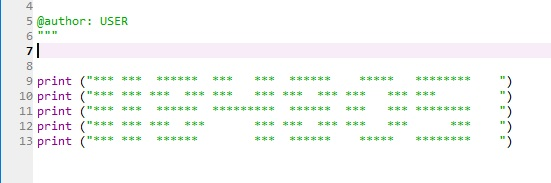
\includegraphics[width=11cm\textwidth]{Figure/1.jpg}
    \end{center}
    \item Soal 2
    \begin{center}
    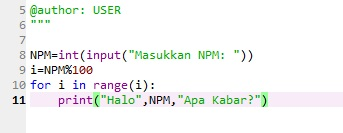
\includegraphics[width=11cm\textwidth]{Figure/2.jpg}
    \end{center}
    \item Soal 3
    \begin{center}
    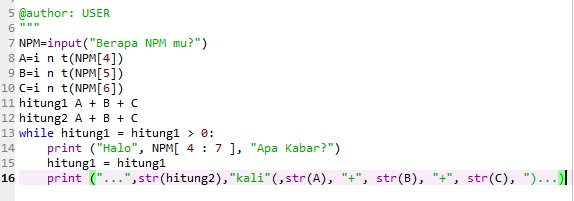
\includegraphics[width=11cm\textwidth]{Figure/3.jpg}
    \end{center}
    \item Soal 4
    \begin{center}
    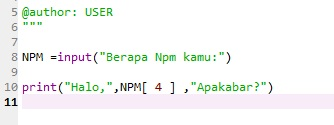
\includegraphics[width=11cm\textwidth]{Figure/4.jpg}
    \end{center}
    \item Soal 5
    \begin{center}
    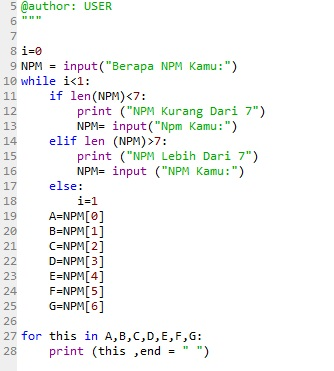
\includegraphics[width=11cm\textwidth]{Figure/5.jpg}
    \end{center}
    \item Soal 6
    \begin{center}
    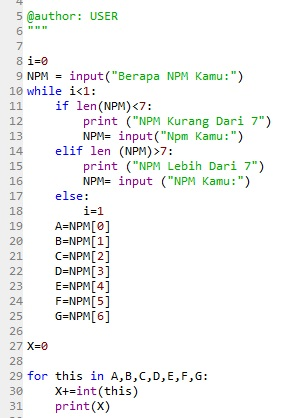
\includegraphics[width=11cm\textwidth]{Figure/6.jpg}
    \end{center}
    \item Soal 7
    \begin{center}
    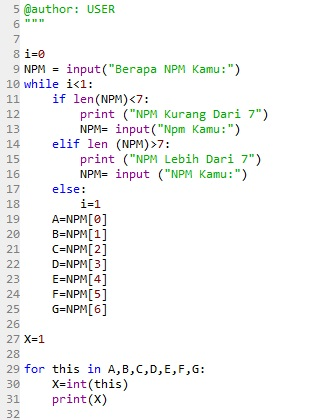
\includegraphics[width=11cm\textwidth]{Figure/7.jpg}
    \end{center}
    \item Soal 8
    \begin{center}
    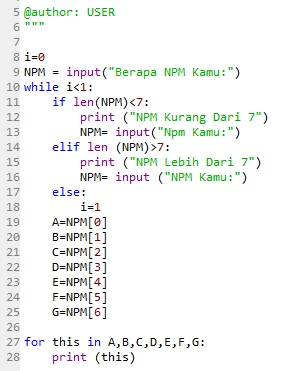
\includegraphics[width=11cm\textwidth]{Figure/8.jpg}
    \end{center}
    \item Soal 9
    \begin{center}
    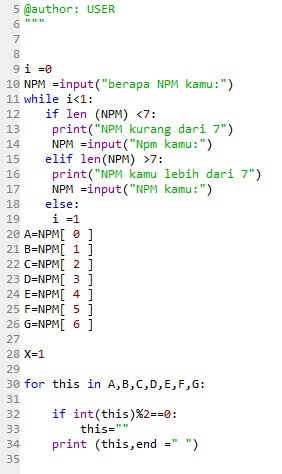
\includegraphics[width=11cm\textwidth]{Figure/9.jpg}
    \end{center}
    \item Soal 10
    \begin{center}
    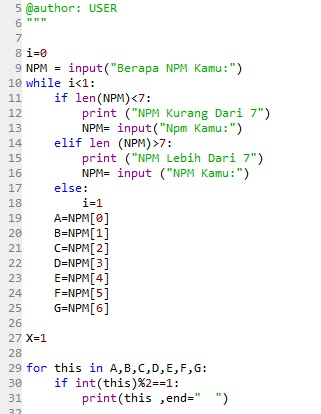
\includegraphics[width=11cm\textwidth]{Figure/10.jpg}
    \end{center}
    \item Soal 11
    \begin{center}
    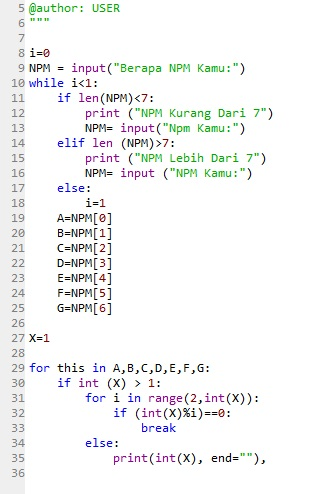
\includegraphics[width=11cm\textwidth]{Figure/11.jpg}
    \end{center}
\end{enumerate}
\section{Penanganan Eror}
    \begin{center}
    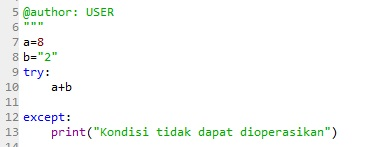
\includegraphics[width=11cm\textwidth]{Figure/err.jpg}
    \end{center}
\item Soal 11
    \begin{center}
    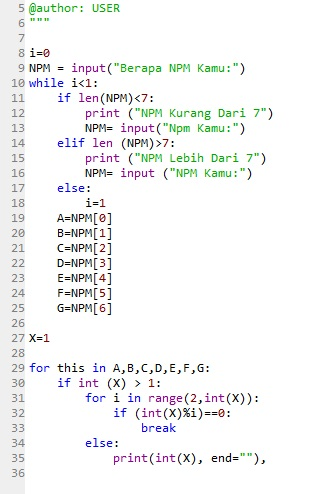
\includegraphics[width=11cm\textwidth]{Figure/11.jpg}
    \end{center}
\end{document}

